\begin{figure}[H]
\caption{Discrete wavelet transform using Haar
filter}\label{figure:haar_transform}
\caption*{\\[0em]\footnotesize\textit{$W1, \ldots, W6$ represent the levels of
decomposition in reversed order, the lower most graph shows the original
signal. The coefficients plotted at $W6$ (top most graph) are generated in the
first step of decomposing. Each level from $W6$ to $W1$ adds detail from the
original signal. The highest level ($W1$) is closest to the original signal. No
more detail is left from the original signal that can be added in any further
step.}\\[1em]}
\centering
	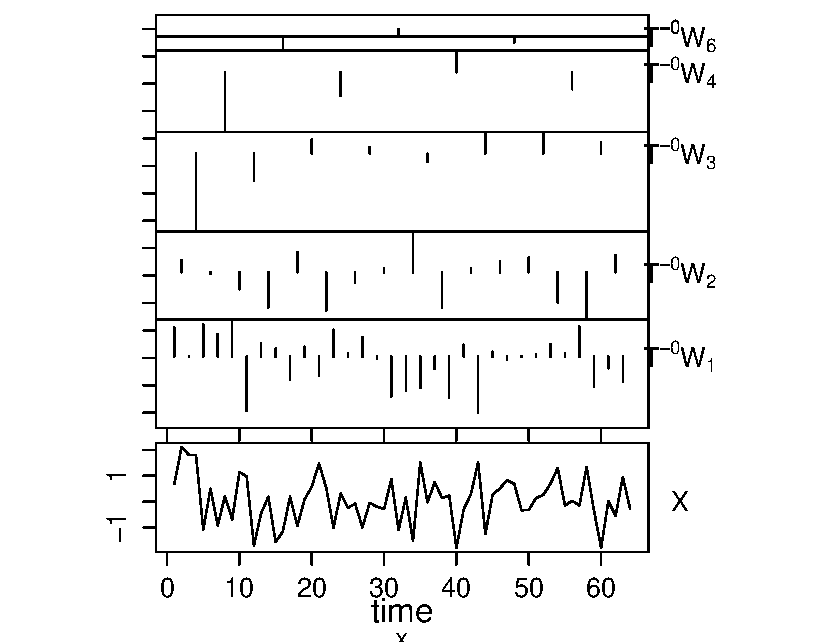
\includegraphics[scale=0.9]{images/dwt_haar.pdf}
\end{figure}